%%%%%%%%%%%%%%%%%%%%%%%%%%%%%%%%%%%%%%%%%%%%%%%%%%%%%%%%%%%%%%%%%%%%%%%%
%                                                                      %
%     File: Thesis_Introduction.tex                                    %
%     Tex Master: Thesis.tex                                           %
%                                                                      %
%     Author: Andre C. Marta                                           %
%     Last modified :  4 Mar 2024                                      %
%                                                                      %
%%%%%%%%%%%%%%%%%%%%%%%%%%%%%%%%%%%%%%%%%%%%%%%%%%%%%%%%%%%%%%%%%%%%%%%%

\chapter{Introduction}
\label{chapter:introduction}

The space race between the United States and Russia was a reality that drove technological advances since then. Reaching the moon was an inherent goal in this competition won by the United States. For years, only government agencies have conducted space missions primarily for scientific purposes. With the demand for space missions, it became necessary to look at space vehicles from a different perspective, with the goal of making them profitable \cite{gomes_road_2013}. An example of this change in the paradigm of space travel is the Space Shuttle programme, a reusable spacecraft that allowed multiple flights and therefore contributed to the construction of the \gls{iss}. However, in recent years, the space race has been dominated mainly by private companies \cite{gomes_road_2013}, as examples SpaceX \cite{noauthor_spacex_nodate}  or BlueOrigin \cite{noauthor_blueorigin_nodate} are two of the most prominent ones, with two different visions about space.

There is currently a slow but steady increase in private companies involved in new space economy \cite{quinn_acceptable_nodate}. There are several causes and/or development reasons for this trend, and technological progress is playing a crucial role in making space travel not only more financially accessible, but also safer \cite{blue_l_2017} echnological advancement also has brought about clear improvements in other areas, such as telecommunications \cite{garzaniti_review_2021}.

Safety issues are critical for proper functioning and sense of space missions to, minimising risk to human life  and cargo loss \cite{quinn_acceptable_nodate}. These safety issues are something NASA has taken into account \cite{shin_nasa_2014}, since the early days of human space travel and more recently other international agencies to improve the risk analysis of space travel.  However, economic chanllenges compel private companies to minimise the operating costs per space mission \cite{gomes_road_2013}. An increase in the performance of both launchers and the remaining stages is inherent and necessary for the expansion of a new space ecosystem that underlies this technological progress \cite{garzaniti_review_2021}. This space ecosystem is  based on launcher systems, space platforms, manufacturing processes, and materials \cite{garzaniti_review_2021}, which form the basis for studies that are currently being conducted.

To address economic challenges, one of the systems that has been extensively studied and becomes crucial during a space mission is the Entry, Descent, and Landing (EDL) system \cite{diaz-silva_rotary_2013}. NASA initially employed parachute systems, figure \ref{fig:thurst-vector}, for the recovery of astronaut capsules \cite{ragab_launch_2015}. Nowadays,  SpaceX \cite{noauthor_spacex_nodate} and many other companies are making efforts onstudies about the use a recovery system based on a controlled thrust vector, as shown in figure \ref{fig:thurst-vector}.

\begin{figure}
    \centering
    \begin{minipage}{.45\textwidth}
      \centering
     \includegraphics[height=45mm]{Figures/introduction/parachute-system.jpg}
      \caption[Parachute recovery system]{Parachute recovery system \cite{noauthor_wikipedia_nodate}}
      \label{fig:parachute-system}
    \end{minipage}%
    \begin{minipage}{.05\textwidth}
         \text{ }
    \end{minipage}
    \begin{minipage}{.45\textwidth}
      \centering
      \includegraphics[height=45mm]{Figures/introduction/rocjet-thrust-vector.jpg}
      \caption[Controlled thrust vector recovery system]{Controlled thrust vector recovery system \cite{noauthor_spacex_nodate}}
      \label{fig:thurst-vector}
    \end{minipage}
\end{figure}

%%%%%%%%%%%%%%%%%%%%%%%%%%%%%%%%%%%%%%%%%%%%%%%%%%%%%%%%%%%%%%%%%%%%%%%%
\section{Autorotation for Space Vehicles}
\label{section:autorotation_vehicles}

Using an unpowered rotary wind as an aerodynamic decelerator for spacecraft recovery from a space mission is not a new concept \cite{diaz-silva_rotary_2013}. More than 80 years ago, the first studies were performed, but rapidly the concepts lost interest. Years after it gained new enthusiasts and some recent projects were published. This section assesses the evolution of the use of Autorotation for Spacecraft.

\subsection{Rotary Wing Recovery System In the Early Ages of Space Exploration}

Over the years some studies have been published focusing on using rotary wings as a concept for vehicle recovery. Ricardo A. Diaz-Silva in \cite{diaz-silva_rotary_2013}, states that early concepts date 1947, when Igor Bensen, from the General Electric Co, published a report titled \textit{Development of Rotochute Rotary Wing Air Brake}. In its work, Bensen developed a device known as Rotochute (Fig. \ref{fig:rotochute_prototype}) which is a result of merging two keywords: rotor and parachute. The main objective of this device was to develop an aerodynamic decelerator for high-altitude rockets. This device was at the time studied at a supersonic wind tunnel to understand reentry effects. 

\begin{figure}[!htb]
    \centering
    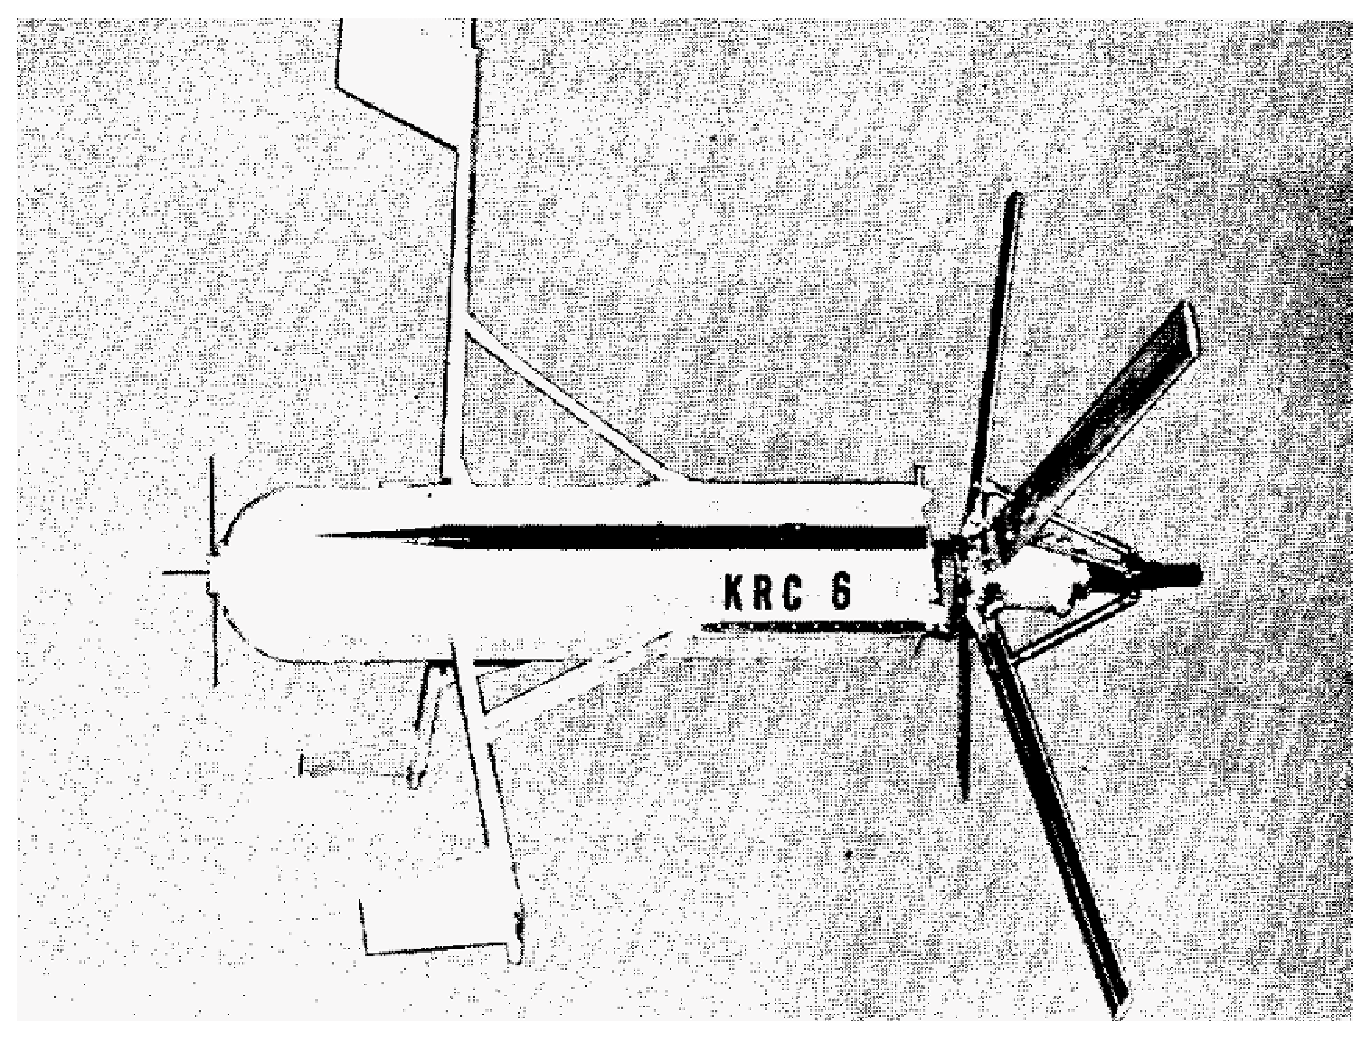
\includegraphics[width=8cm]{Figures/introduction/rotochute_prototype.eps}
    \caption{KRC-6 Rotochute Flight Test Vehicle}
    \label{fig:rotochute_prototype}
\end{figure}

Also, Kaman Corporation \cite{noauthor_kaman_nodate} got involved in the rotochute design in the 50's decade and the \gls{nasa} spent some attention studying the proposed system in the 60's, never putting it into practice once all Apollo Missions \cite{noauthor_apollo_nodate} were accomplished by recovering the crew capsule with parachutes landing on the ocean. Important authors in this decade working on the topic, cited in \cite{diaz-silva_rotary_2013}, were Rodney Wernicke from the Bell Helicopter Company, 1957, Justin J. Barzda from Kaman Corporation, 1964, and M. Kretz from the Giravions Dorand Co. in France, 1966. These authors made a substantial original contribution to the area, it is important to comprehend the main ideas of this system by providing a brief overview of their work.

Wernicke published \textit{Preliminary Tests of Model Spacecraft Rotor Landing System} \cite{wernicke_preliminary_1959} where a three-bladed model was used as able to reduce the vehicle descent axial velocity from supersonic regime to subsonic glide. In its work, Wernicke studied the influence of collective pitch on the model's performance.

On the other hand, Barzda published \textit{Rotor for Recovery} \cite{barzda_rotors_1964} were fixed and telescoping span blades, rotor diameters ranging from 0.3 to 7.3 \unit{m}, payloads 2.7 to 408 \unit{kg}, and rates of descent as low as 6 \unit{m/s} were points of experimental tests. Barzda did the experimental investigation of deployment from jet aircraft and from a cannon-fired flare shell at  Mach numbers 0.98 and 1.2, respectively. From this investigation, drag and lift coefficients, glide ratios, and cyclic and collective flare performance were crucial results, necessary for the advancement of the concept.

\textit{Space Rotor: A European Project for Recovery of Heavy Launch Vehicles} \cite{kretz_space_1966} was published by Kretz and registered a patent. His design aimed to help spacecraft return from orbit by using rotors that could be deployed before re-entry. The system offered benefits like better flight stability, longer range, and precise, soft landings, making reusable launch vehicles possible.

From a historical perspective, Diaz-Silva \cite{diaz-silva_rotary_2013} also makes reference to a Sovietic interest in this system for its Soyuz capsule recovery system, but no references can be found.


\subsection{Why using rotary wings for space vehicle recovery?}

To understand why using a rotary wing is a key advantage in space exploration, one can get back to Barzda (1964) \cite{barzda_rotors_1964} where it is answered. This analysis is mainly done by connecting an already known application of autorotation: helicopters autorotation mandatory manoeuvre in case of power losses \cite{federal_aviation_administration_helicopter_2021}. As helicopters, this is a weatherproof system that can perform under icing or stormy conditions. Another important advantage is the fast and precise deployment over a wide range of speeds. Retardation force builds up rapidly when body orientation is adequate. This allows for recovery, for example, the launcher, when it is necessary to abort the mission in the middle flight to save human lives or payload. A rotary wing is a controllable system, meaning that the pilot or a flight computer can control the vehicle trajectory and rate of descent \cite{federal_aviation_administration_helicopter_2021}. This is an important feature of this system once it is possible to make a safe landing at the intended landing site.

Also over the traditional, parachute, and nowadays in-development technology, \gls{tvc}, using a rotary wing under autorotarion phenomena has some advantages. Marques (2022) \cite{marques_rocket_2022}, present a table comparing four different recovery technologies showing an outstanding advantage over the parachute and a good advantage over \gls{tvc}. Another table was presented by Steiner \cite{steiner_rotary_nodate} who also used as a recovery methods comparison criterion the unpowered advantage of the autorotation system, showing that the rotary wing is also more efficient in terms of recovery systems


Over the parachute system, cost and weight are the major drawbacks, but controllability is something that a rotary wing deccelerator would provide \cite{steiner_rotary_nodate}. Relatively to \gls{tvc}, the rotary wings system presents the possibility of controlled gliding, mission flexibility and a wider range of applications. For \gls{tvc} is also needed extra fuel and larger space launcher which increases the power for the mission's launch phase. Clearly, the rotary wing system is a good option for space vehicle recovery.

%%%%%%%%%%%%%%%%%%%%%%%%%%%%%%%%%%%%%%%%%%%%%%%%%%%%%%%%%%%%%%%%%%%%%%%%
\section{Autorotation Overview}
\label{section:overview}

A rotor's ability to spin even in the absence of motor power is known as auto-rotation, an aerodynamic phenomena that enables a controlled landing \cite{steiner_rotary_nodate}. The movement of air via the rotor's blades powers it. When this airflow hits the rotor's inclined blades, it creates lift force, which keeps the vehicle in the air. Important factors in producing this force are the rotor blades' angle and the pressure difference between their upper and lower surfaces.

Note that auto-rotation is not the same as free flight. In auto-rotation, a controlled descent is occurring, and the pilot must constantly adjust the angle of the rotor blades to maintain balance and control the rate of descent \cite{federal_aviation_administration_helicopter_2021}. Numerous variables, including the helicopter's weight, height, air temperature, humidity, and wind speed, affect how effective auto-rotation is.


\subsection{Helicopters Autorotation Maneuver}

When it comes to helicopter emergency manoeuvres, autorotation is one of the most important skills that pilots use in the event of a failure of the engine \cite{federal_aviation_administration_helicopter_2021}. This method uses a controlled fall that starts with reducing the collective pitch control \cite{federal_aviation_administration_helicopter_2021}. Then it uses upward airflow to provide lift, maintain rotation of the rotor  blade, and postpone descent. To maintain control throughout the manoeuvre, the pilots adjust the direction  and attitude of the helicopter using cyclic control. The pilot performs a flare, further slowing the descent  velocity as the helicopter gets closer to Earth by lowering the collective a little. Because auto-rotation is a skill that is acquired via extensive training, it is a dependable way for pilots to land safely in the event of unplanned power outages, which greatly enhances aviation safety in general.

 \begin{figure}[!htb]
    \centering
    \includegraphics[width=7cm]{Figures/introduction/helicopter maneuver.png}
    \caption{Stages of helicopter emergency landing maneuver: 1) engine failure; 2) autorotation descent; 3) flare manoeuvre; 4) approaching landing site; 5) landing}
    \label{fig:helicopter-maneuver}
\end{figure}

\subsection{Projects and literature review}

In recent years, new developments have been published about using rotary wings for recovery space vehicles. The publications show completely different results from the early concepts once the computation technologies have also evolved over the years. It allows researchers to gain deep knowledge of the autorotation phenomena throw computational simulations. Also, conceptual model vehicles were possible to be built with onboard computers to get data from experimental flights due to electronics development.

\subsubsection{ARMADA}

A fundamental state-of-the-art project was started to be developed in 2008  by the \gls{esa}, GMV, the University of Bologna and the European Aeronautic \gls{EADS}. The so-called \gls{armada} project \cite{noauthor_armada_nodate} is an \gls{edls}. Its relevance in the field is significant once many other projects were published and taken as reference \gls{armada} project. 

 In the proposed system of \gls{armada} (Fig \ref{fig:armada_concept}) a rotor is connected to a conventional helicopter control system, which in turn is mounted on the structure that supports the payload. The deployment process occurs in several stages. Initially, body flaps extend to stabilize the vehicle during deployment. Following this, the rotor blades are deployed using a cable to minimize stress on the joints. 

\begin{figure}[!htb]
    \centering
    \includegraphics[width=8cm]{Figures/introduction/armada_concept_vehicle.png}
    \caption{ARMADA Autorotation system concept, from \cite{noauthor_armada_nodate} }
    \label{fig:armada_concept}
\end{figure}

During the deployment, the blades are set to a zero-lift configuration to prevent rotation, with an additional braking system on the rotor shaft ensuring no movement. Once the blades are fully deployed, the retention cables are released, the rotor brake is disengaged, and the collective pitch of the blades is adjusted to allow the rotor to spin. As the lander crosses a predetermined Mach number, centrifugal force extends the telescopic blades, which were initially held in a retracted position by a cable. From this point, the lander descends in its fully deployed state, reaching an equilibrium descent velocity. Just before landing, a flare manoeuvre is executed to further reduce both vertical and horizontal velocities for a safe touchdown.

In \cite{noauthor_armada_nodate}, the deployment phase is further addressed by considering different types of rotor deployment systems. Using a single-piece blade rotor is small and suitable for thicker atmospheres, while a telescopic blade rotor features extendable sections for easy deployment using internal cables. Inflatable blade rotors are lightweight and compact but store less kinetic energy, limiting their manoeuvrability. Foldable blade rotors require precise locking mechanisms to ensure structural stiffness and flexible blade rotors are stabilized through reefing lines, stiffeners, or centrifugal forces in their deployed state. To achieve the best deployment, \textit{"Any deployment system that can modify the blade length in-flight is highly desirable since this allows an easy method of reefing."}, as the authores state, proposing more suitable telescopic blades.

\gls{armada} \cite{noauthor_armada_nodate} concepts performance is done using simulations and wind tunnel experiments. Starting with the software tools, Fig. \ref{fig:armada_software}, uses a divide and conquer approach in which a Performance Database (PD) and an Integrated Parametric Design  Tool (IPDT). To resume how it works, de PD is in simple words a tabe with rotor parameters under specific conditions and de IPDT is interface sheets that interact with the database.

\begin{figure}[!htb]
    \centering
    \includegraphics[width=6cm]{Figures/introduction/armada_software.png}
    \caption{ARMADA concept software, from \cite{noauthor_armada_nodate}}
    \label{fig:armada_software}
\end{figure}

For the experimental tests \cite{noauthor_armada_nodate}, a small-scale model, presented in Fig. \ref{fig:armada_windtunnel} is used. For the supersonic deployment model, figure \ref{fig:armada_supersonic_model}, the S-1 supersonic/transonic wind tunnel 
at Von Karman Institute of Fluid Dynamics was used to test it to Mach number up to 2. For the subsonic regime, the model is tested in the wind tunnel of the Applied Aerodynamic Laboratory of the University of Bologna.

\begin{figure}[!htb]
    \centering
    \subfloat[Supersonic deployment model\label{fig:armada_supersonic_model}]{
        \includegraphics[height=6cm]{Figures/introduction/armada_supersonic_model.png}
    }\hfill
    \subfloat[Subsonic reefing model\label{fig:aircraft2}]{
        \includegraphics[height=6cm]{Figures/introduction/armada_subsonic_model.png}
    }
    \caption{ARMADA concepts under different fight conditions, from \cite{noauthor_armada_nodate}}
    \label{fig:armada_windtunnel}
\end{figure}

As results of the study \cite{noauthor_armada_nodate}, show an equilibrium descent velocity that can be obtained with the type of design presented is about 30-40 \unit{m/s} and was found that this terminal velocity cannot be reduced by increasing the rotor size, and the mass of the rotor itself becomes an important contributor to the overall mass of the vehicle. About this point an essential remark is made:  the mass of the recovery system remains attached to the vehicle, but in traditional systems some mass gets ejected (parachutes) or burnt (propellant). In terms of aerodynamic performance, the distinction between stalled and unstalled operation is evident in the rotor drag coefficient and descent velocity. In installed conditions, the rotor drag coefficient ranges from 1 to 1.25, with a descent velocity of approximately 31 \unit{m/s}. Conversely, when stalled, the rotor drag coefficient drops to around 0.25, and the descent velocity increases significantly to about 80 \unit{m/s}. Furthermore, \gls{armada} faces mechanical challenges, including rotor mass, complexity, descent velocity, and vibration issues. Future solutions may involve improved materials and structures, integrated control systems, and the consideration of additional braking mechanisms.

ARMADA's \cite{noauthor_armada_nodate} performance does not justify short-term adoption compared to traditional \gls{edls}. Further research on these approaches is necessary. Overall, ARMADA presents a promising alternative for EDL systems on Earth, Venus, or Titan in the medium to long term.



\subsubsection{Hummingbird}

Further investigation takes to another conceptual project. An undergraduate research project called Project Hummingbird \cite{maurer_project_nodate} aims to launch and recover a sounding rocket with a safe landing achieved by a rotor recovery mechanism. The effort aims to introduce a novel approach to booster recovery that minimizes fuel requirements, streamlines the system, and lowers launch costs.

With foldable rotor blades and an internally stored rotor hub, the system is designed to launch to a height of 2,700 meters. A little parachute will pop out of the nose cone's tip at apogee, allowing the rocket to be oriented with its nose facing upwards. The nose cone will separate in its entirety upon correct alignment. The rotor blades will then immediately deploy and start to revolve on their own, slowing the rocket's descent speed. The rotor will execute a flare movement as the rocket gets closer to the ground to guarantee a safe landing. There will be a flight computer monitoring the rocket's direction and fall. If the rotor blades fail to sufficiently slow down the drop, an emergency parachute will deploy.

\begin{figure}[!htb]
    \centering
    \includegraphics[width=10cm]{Figures/introduction/Hummingbird_operation.png}
    \caption{Concept of Operation of Project Hummingbird, from \cite{maurer_project_nodate}}
    \label{fig:Hummingbird_operation}
\end{figure}

This project \cite{maurer_project_nodate} demonstrates an alternative application of rotary wings as a recovery system and introduces a useful hybrid system that combines parachutes and rotary wings. This combination could be crucial if the vehicle is not in the correct position during rotor deployment. Additionally, higher velocities during the deployment phase may result in increased structural stresses, as noted in \cite{noauthor_armada_nodate}.

\subsubsection{DEADALUS}

Riegler et al. developed a prototype \cite{riegler_daedalus_2018} aiming for Earth atmospheric research but also for other \gls{leo} missions. In this work, the authors state that new and safe technologies are needed in the field, proposing a self-stabilizing, free-falling unit, capable of measuring and distributing atmospheric data during descension \cite{riegler_daedalus_2018}. For accomplished the teams goal's, they started by develop the rocket prototype called REXUS, presented in Fig. 3. 


\begin{figure}[!htb]
    \centering
    \includegraphics[width=10cm]{Figures/introduction/REXUS-Rocket-composition_W640.jpg}
    \caption{REXUS Rocket composition, from \cite{riegler_daedalus_2018}}
    \label{fig:rexus_rocket}
\end{figure}

On the REXUS prototype \cite{riegler_daedalus_2018} a set o  \gls{ffu} so called SpaceSeeds, are placed inside the REXUS cone, figure \ref{fig:ffu_rexus_inside} and will be injected once the rocket reaches its apogee. This SpaceSeeds are the intereste key point of DEADALUS project on the scope of the use of rotary wings under autorotation phenomena as a recovery system for spacecraft. Figure \ref{fig:ffu_rexus_model} presents a SpaceSeed prototype is presented with four-bladed rotor and a conical main body.



\begin{figure}[!htb]
    \centering
    \subfloat[SpaceSeeds placement inside REXUS's cone, from \cite{noauthor_daedalus_nodate}\label{fig:ffu_rexus_inside}]{
        \includegraphics[height=7cm]{Figures/introduction/ffu_rexus.png}
    }\hfill
    \subfloat[SpaceSeed protoype, from \cite{riegler_project_nodate}\label{fig:ffu_rexus_model}]{
        \includegraphics[height=7cm]{Figures/introduction/space_seed_prototype.png}
    }
    \caption{\gls{ffu} SpaceSeeds used in DEADALUS project}
    \label{fig:daedalus_ffu}
\end{figure}

The development and construction of the space are further presented by Riegler et al. in \cite{riegler_project_nodate}. In this study, the authors explain in better detail the aerodynamic characteristics and software and telemetry information and electronics and its \gls{orbc}. Using the paper words \cite{riegler_project_nodate}, the \gls{orbc} is the interface between the \gls{rxsm} and the SpaceSeeds, so it is important to refer to it. 

Another important aspect of the project is the mechanical setup. Although it is not the main subject of this study, it is important to highlight the necessity of other components in \cite{riegler_project_nodate} technology. Related to this work two key points are presented: the deployment mechanism which is a crucial aspect of the project once it is necessary to separate the SpaceSeeds from the launcher; the second important point is the wings folding mechanism. The latest mechanical components are not a key point for this study, but it is important to take into consideration, that for spacecraft recovery the blades must be kept inside the vehicle during the launch phase. The blades should only open, unfold or any other way of deploy during the descent phase.

For the mechanical setup, the authors \cite{noauthor_daedalus_nodate} found some mechanical challenges that one must take into consideration: flight loads, especially in the transonic regime, minimum weight, volumetric constraints, natural aerodynamic stability, antenna positioning, radio translucent materials at corresponding areas and landing shock loads.

Finally and more important, is the flight tests. In \cite{riegler_project_nodate} the authors presented a set of different simulation and real flight tests showing good accuracy from computational model and real-flight data. A deeper look at this data is taken in section \ref{sec:validation_verification} in which the data is used to validate the computational model presented in this.

From the same authors \cite{mehringer_suborbital_2022} and \cite{bergmann_daedalus_2024} are two more recent publications about the DEADALUS project, in this case, the second version. In thiese papers, some improvements are made to the setup but no available data is presented for comparison.


%%%%%%%%%%%%%%%%%%%%%%%%%%%%%%%%%%%%%%%%%%%%%%%%%%%%%%%%%%%%%%%%%%%%%%%%
\section{Autorotation Analysis Methodologies and Literature Review}
\label{section:literature_review}

The autorotation phenomena is a wide study phenome from the 1923 when Juan de la Cierva built the Autogiro \cite{leishman_principles_2006}. The autogiro was a rotary-wing type aircraft caple of flying at low speed and landing in short runways. Over the next 15 years, de la Cierva develop is Autogiro concept proving a very safe air transportation system. On the other way, the Bell Hellicopter Corporation, 1959, was the first to publish \cite{diaz-silva_rotary_2013} some work about the studyies of Autorotation for helicopters safety maneuver. However, there is no online access to their works to understand their methodologies, models and resutls. 

But one can return to the begin of the  20th Century when Nikolsky (1906) \cite{nikolsky_analytical_1906} publish one of the first, or even the first, article about 
a rotary wing performance under a descent trajectory. This study considered the major aerodynamic effects know to the time as induced velocity, blade stalling and pithc angle. As a key contribution for the rotary wing evolution, for small blade incidence angles, autorotation remains sufficiently stable, and blade stalling can be neglected. However, as the incidence increases, the risk of an upgust inducing stall and halting the rotor becomes significant. Also, before the era of computers, all Autorotation studies were performed using wind tunnels. \cite{smith_autorotating_1971} studyied,, in The University of Michingan's wind tunnel the Autorotation phenomena of a flat plate measuring the basic aerodynamic proprieties and angular momentum for a wide number of Reynolds, $Re$. 


Now a days, the computer capabilities opens a window to dig deep into the Autorotation with computational models and fast numeric tools. Marques (2022) \cite{marques_design_2024} as shown the feasibility of using rotary wings as a recovery system for spacecraft, but the study was limited an axial descent with a very-low fidelity model. Riegler et al. (2018) \cite{riegler_daedalus_2018} has also study autorotation in high altitudes considering also an axial descent trajectory. In axial flight there is much more investigation as Cuerva (2006) \cite{cuerva_engineering_2006} , Nadal Mora et al. (2005, 2006, 2007) \textcolor{blue}{falta as referências}. Kim (2009) \cite{kim_v_2009} also study the autorotation but with focus on a forward flight. Brindejonc (2007) \cite{brindejonc_design_2007} published a recent wind tunnel test to conducted a parameteric study for rotor proprieties. Czyż (2021) \cite{czyz_v_2021} study the transient behaviour of a rotor under a constant flow field using \gls{cfd} tools.

%%%%%%%%%%%%%%%%%%%%%%%%%%%%%%%%%%%%%%%%%%%%%%%%%%%%%%%%%%%%%%%%%%%%%%%%
\section{Objectives}
\label{section:objectives}

Although autorotation is a industry standard for helicopters, the use of rotary wings under autorotation phenomena as a recovery system for spacecraft is still in its beginning. The main objective of this study is to investigate the feasibility of using rotary wings as a recovery system for spacecraft, with a focus on the autorotation phenomena. Also, for a spacecraft which comes from \gls{leo} or the outer space, the altitudes, velocities and atmospheric proprieties under which the system will operate are not the same as those of helicopters. Therefore, the study aims to investigate the effects of Autorotation in high altitudes, over helicopter flight ceiling.

Hence, this study will explore alternative approaches beyond those presented in \ref{section:literature_review}. The primary engineering objective is to develop a simulator capable of predicting the performance of a rotary-wing system undergoing autorotation at higher altitudes than in previous work \cite{marques_design_2024}. At these altitudes, the significantly lower atmospheric density is expected to delay the onset of autorotation. The simulator will also be used to analyze the influence of various rotor geometric properties on system behavior.

Furthermore, the dynamic \gls{6dof} model is introduced by incorporating an additional aerodynamic model optimized for faster computations, improved numerical solvers, and aerodynamic considerations such as tip losses. As a crucial factor, the simulator must be able to show the rotor aerodynamic loads and simulation proprieties for a time step for the entire disk. This will further help on visualizing the rotor performance and verify the simulation.

Finally, a key objective of this study is to simulate the system's response under the influence of wind gusts. Wind will be used as the perturbation phenomena to the rotor performance and will be a critical study either the feasibility and controllability of the system.

%%%%%%%%%%%%%%%%%%%%%%%%%%%%%%%%%%%%%%%%%%%%%%%%%%%%%%%%%%%%%%%%%%%%%%%%
\section{Thesis Outline}
\label{section:outline}
